%\documentclass[JIP,draft]{ipsj}
%\documentclass[JIP]{ipsj}

\documentclass[JIP]{apris}

\usepackage[dvips]{graphicx}
\usepackage{latexsym}

\def\Underline{\setbox0\hbox\bgroup\let\\\endUnderline}
\def\endUnderline{\vphantom{y}\egroup\smash{\underline{\box0}}\\}
\def\|{\verb|}

\setcounter{volume}{20}% vol20=2012
\setcounter{number}{4}% 1, 2, 3, 4
\setcounter{page}{1}

\received{2011}{7}{1}
%\rereceived{2011}{10}{1}   % optional
%\rerereceived{2011}{10}{31} % optional
\accepted{2011}{11}{5}

\usepackage[varg]{txfonts}%%!!
\makeatletter%
\input{ot1txtt.fd}
\makeatother%

\begin{document}

\title{code2vec for C: The Acquisition Method of Distributed Representation of the C Language with The TF-IDF Method}

\affiliate{IPSJ}{Faculty of Information Science and Electrical Engineering, Kyushu University}
\affiliate{JU}{Graduate School of Information Science and Electrical Engineering, Kyushu University}
\affiliate{F}{Fujitsu Kyushu Network Technologies Limited}

\author{Kotori Hieda}{JU}[hieda@f.ait.kyushu-u.ac.jp]
\author{Kenji Hisazumi}{IPSJ}[nel@slrc.kyushu-u.ac.jp]
\author{Hirofumi Yagawa}{F}
\author{Akira Fukuda}{IPSJ}[fukuda@f.ait.kyushu-u.ac.jp]


\begin{abstract}
Code2vec is a method for obtaining a distributed representation of program code. It obtains the embedding vector of program code through machine learning and predicts the label such as ‘method body’ representing the functionality of the code snippets. Thus, it is possible to obtain a distributed representation of the code snippet whose meaning is taken into account. In embedded system development, the non-object-oriented programming language C is often used, however code2vec is intended for object-oriented programming languages such as Java and C\#. Therefore, to apply code2vec to the C language, there are some problems that must be solved: labelling is difficult since the function name differs from that of the object-oriented language, and we need to develop a method of feature amount extraction from C language. In the following paper, we propose a method for extracting feature values from the C language programs and making use of the TF-IDF method for decomposing a given function name into both module-specific names and general operation names, as found in object-oriented languages.
\end{abstract}

\begin{keyword}
code2vec, TF-IDF, C language, code snippet, function name estimation
\end{keyword}

\maketitle

%1
\section{Introduction}
In natural language processing, methods for obtaining distributed representations that take into account their meanings such as word2vec\cite{rong2014word2vec} have been proposed and applied in various ways. Current software development is supported in various ways using similar methods in program code, however there is room for improvement in both methods and applications. 

Code2vec\cite{alon2019code2vec} has been proposed as a method for obtaining the distributed representation of a given program’s code. In this approach, it is possible to numerically express the code snippets and the relationship between them as real vectors. The main application of the distributed representations obtained by code2vec is to estimate the method name from the method body. Code2vec is designed for object-oriented languages such as Java and C\#. 

C language is often used in embedded systems, however, as it is not an object-oriented language, it is not possible to directly apply C language to code2vec. In particular, when estimating the function name, estimation accuracy decreases because the function name itself contains both the module-specific name and general operation name.

In this study, we apply TF-IDF (Term Frequency Inverse Document Frequency)\cite{ramos2003using} to the function name to remove module-specific names based on the TF-IDF value as shown in Table~\ref{table1}. The TF-IDF value increases when a certain word appears frequently in a specific document, whilst only appearing infrequently in other documents. Since the module-specific name is unique within a document, its TF-IDF value is high. Therefore, we set a threshold for the TF-IDF value and delete the one with the highest value to leave only the operation name. By learning only operation names as function names, we aim to improve the accuracy of function name estimation. 

\begin{table}[t]
 \centering
 \caption{Result of using TF-IDF method}
 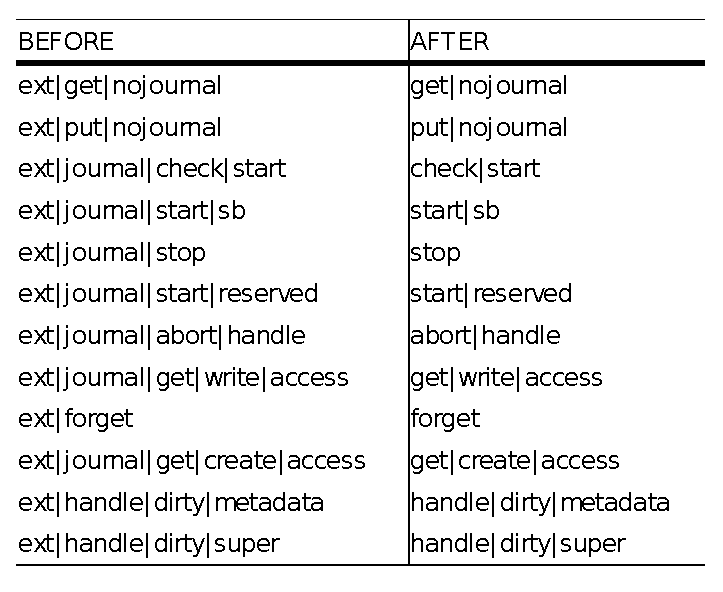
\includegraphics[width=1.0\hsize]{image/ITF-DFcompare.eps} 
 \label{table1} 
\end{table}


%2
\section{Related research}
The CMU-SEI group\cite{code2vec-c} implemented a C parser for code2vec.
% Cmu-sei\cite{}の研究では、我々と似たような手法でC言語へのcode2vecの適用を試みていた。
They paid attention to syntactic differences between parsers of C and Java, such as function declarations in C are not in Java.
They used Clang and LLVM\cite{lattner2007clang}, and tried to apply code2vec to C language by abstracting the functions.
% 彼らはCとJavaのパーサーの違いや、Cにある関数宣言がJavaにはないことなどに着目し、我々と同様にClangとLLVMを使用し、関数を抽象化することで、code2vecのC言語への適用を試みていた。
In this case, the accuracy of function name estimation may not improve because the module name and operation name are not separated.
% しかし、彼らはTF-IDFを用いていない。これではモジュール名と操作名が分離されていないので、関数名推定の精度が上がらない恐れがある。そこで我々は彼らとTF-IDFを用いた我々での関数名推定の制度を比較し検討した。


%3
\section{Analytical method}
In this section, we describe the analysis procedure of C language program code.
Since a C language program is made up of a plurality of files, it performs the processing for each file. First, it extracts a function definition. A function definition consists of a function name, arguments, return value, and function body.

The function name is usually a compound word, so we extract only the general terms. Since camel case and underscore are used to represent word breaks, we extract words by separating them.
Besides, numerical values ​​are often inappropriate as general words, so we delete them. We do them for all prepared C language programming code files.

 We calculate all occurrences number of documents about a word (DF) and consider this as an entire dictionary. We also make a dictionary about the frequency of appearance of each word (TF) for each file. Based on these dictionaries, we calculate the TF-IDF value.
We calculate the TF-IDF value of a word X in document A as (frequency of word X in document A) / (total frequency of all words in document A) * log (total number of documents) / (number of documents containing word X).
After calculating all the words' TF-IDF, it makes a function name with the deletion of words below the threshold.

 Next, we extract features from the function body and analyze code2vec following other language's implementation method.
We parse the function body, convert it to an abstract syntax tree, and extract all terminal symbols in the tree.
We consider all combinations of the extracted terminal symbols and extract a sequence of non-terminal symbols and terminal symbols connecting terminal symbols as a path.

 Code2vec learns the function name consisting of only common words and the feature value extracted from the function body.


%4
\section{Result}
Table~\ref{table2} shows a comparison of the results of CMU-SEI and our function name estimation.  
We compare the top 50 repositories about C language on GitHub as learning data. According to this, it found that CMU-SEI had better accuracy. 
The reason for this is that CMU-SEI considers the difference between C and Java in 6 major elements, and implements it considering the differences.\\
% 表~\ref{table2}はCMU-SEIと我々の関数名推定の結果の比較である。今回我々はGitHubのC言語のレポジトリのうちトップの50レポジトリを学習データとして比較している。これによるとCMU-SEIの方が精度が良いことがわかった。この理由として、CMU-SEIはCとJavaの違いを6つの要素に分けて考え、その差分に従い実装したためだと考えられる。
1. The C parser uses a simpler maximum leaf node metric beyond which it will skip a function.\\
2. The C parser has a parameter that can be set that determines whether to tag or discard function declarations when they are encountered.\\
3. The C parser does not numbers child nodes and includes this information in the generated code paths.
4. The C parser uses a sha256 hash code.\\
5. The C parser is more permissive and will only filter out symbols, some of which will break file formats.\\
6. The C parser collects all bags of path contexts into a single unique list, shuffles the list, and then samples the datasets (test, val, train) from the shuffled list.
% 1. Cパーサはそれを超えると関数をスキップする、より単純な最大リーフノードメトリックを使用している。
% 2. Cパーサにある関数宣言によって、それが検出された時にタグをつけるか破棄するかを決定するパラメータを設定できる。
% 3. Cパーサは子ノードにつけた番号の情報を生成したコードパスに含めない。
% 4. Cパーサはsha256ハッシュコードを使用している。
% 5. CパーサはJavaと異なり、シンボルのみを除外して残りをリーフノードに残す。
% 6. Cパーサはパスコンテキストのすべてのすべてのバッグを単一の一意のリストに収集し、リストをシャッフルし、そこからデータセットをサンプリングする。

I think that CMU-SEI had better accuracy because of the implementation considering these factors.
So we will try applying TF-IDF to the research of CMU-SEI to given better results.
% これらを考慮した実装を行なったためCMU-SEIの実装の精度がよかったのではないかと考える。
% したがって、我々はCMU-SEIの研究にTF-IDFを適用させればより良い結果になるのではないかと考える。


%5
\section{Conclusion}
%  The code2vec In this research to apply the C language, illustrated the implementation of extracting a feature quantity using LLVM and Clang\cite{lattner2007clang}. In the task of estimating the function name from the function body, an identifier such as C language function name, since it is often composed of compound words and module specific name and general operation name, the time of learning we discussed that there is likely to be an obstacle. Furthermore, in order to solve this problem, we proposed a method of classifying the module-specific names and operation names using the function name of the C language TF-IDF. The results show that it is possible to extract only general operation name from the function name in the C language.
In this paper, we showed how to extract features using LLVM and Clang to apply code2vec to C language.
In tasks that estimate function names from function bodies, identifiers such as C language function names are often composed of compound words consisting of module-specific names and general operation names so we argued that this could be an obstacle.
To solve this problem, we proposed a method for classifying function names in C language into module-specific names and operation names using TF-IDF.
As a result, we found that we can extract only general operation names from function names even in C language.
% 本研究ではcode2vecをC言語に適用すべく,LLVMとClangを用いて特徴量を抽出する実装について示した.また,関数本体から関数名を推定するタスクにおいては,C言語の関数名などの識別子は,モジュール固有名と一般的な操作名との複合語で構成されることが多いため,学習の際に障害になる可能性があることを議論した.さらに,この問題を解決すべく,C言語の関数名をTF-IDFを用いてモジュール固有名と操作名に分類する手法を提案した.その結果,C言語においても関数名から一般的な操作名のみを抽出することができることを示した.
Future challenges include applying TF-IDF to the research of CMU-SEI, the evaluation by applying the proposed method and applying to other identifiers such as variable names and function names. We hope we can finally infer the function from the function name.
 % 今後の課題としては.CMU-SEIの研究へのTF-IDF手法の適用、提案手法を適用することによる評価,関数名のみではなく変数名等の他の識別子への適用による評価などが挙げられる.
 % また最終的には関数名から関数を推定する手法の検討が望まれる。

\begin{table}[t]
 \centering
 \caption{Comparison between CMU-SEI and Kyushu University}
 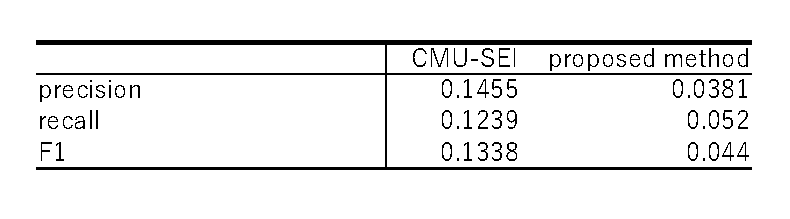
\includegraphics[width=1.0\hsize]{image/cmu-kyu.eps} 
 \label{table2} 
\end{table}


\bibliographystyle{ipsjunsrt}
\bibliography{ebibsample}

% \begin{thebibliography}{99}
% \bibitem{companion}%1
% Goossens, M., Mittelbach, F., and Samarin, A.:
% {\it The LaTeX Companion},
% Addison Wesley, Reading, 
% Massachusetts (1993).

% \bibitem{latex}%2
% Lamport, L.: 
% {\it A Document Preparation System {\LaTeX} User's Guide \&
% Reference Manual}, 
% Addison Wesley, Reading, Massachusetts (1986).
% \end{thebibliography}


\end{document}
